\section{Introducción}

Los grandes modelos de lenguaje (LLM, por sus siglas en inglés) han transformado la manera en que interactuamos con la información. Sin embargo, servirlos de forma eficiente presenta desafíos significativos: la latencia de inferencia es alta (en CPU puede superar los 6 segundos por petición), una única instancia es un punto único de fallo, y sin mecanismos de memorización se repite trabajo ya realizado ante preguntas idénticas o similares.

En este trabajo abordamos estos problemas construyendo una \textbf{granja de modelos de IA} que combina tres pilares fundamentales: \textit{replicación de instancias de inferencia}, \textit{balanceo de carga} y \textit{caché semántico}. El sistema se despliega mediante Docker Compose y está compuesto por cinco servicios: dos instancias de Ollama para inferencia con el modelo \texttt{qwen3.5:0.8b}, una instancia de Ollama dedicada a embeddings con \texttt{nomic-embed-text}, un gateway LiteLLM que actúa como punto de enrutamiento y gestor de caché, Redis Stack como almacén del caché semántico vectorial, y Nginx como proxy inverso de entrada.

La novedad principal del trabajo reside en el uso de caché semántico: en lugar de limitarnos a servir respuestas idénticas desde caché (caché exacto), empleamos Redis con búsqueda por similitud coseno sobre embeddings para detectar preguntas parafraseadas y devolver la respuesta almacenada. Los resultados muestran una aceleración de \textbf{191.5$\times$} en latencia para aciertos de caché (31 ms frente a 5929 ms) y una distribución de carga equilibrada entre las instancias de inferencia.

El resto del documento se organiza como sigue: la Sección~2 presenta los fundamentos teóricos de cada tecnología empleada; la Sección~3 enumera los objetivos del proyecto; la Sección~4 describe la arquitectura del sistema; la Sección~5 detalla la implementación; la Sección~6 analiza el rendimiento mediante experimentos; y la Sección~7 recoge las conclusiones y líneas de trabajo futuro.

\section{Fundamentos teóricos}

\subsection{Docker y Docker Compose}

Docker~\cite{dockerOverview} es una plataforma de contenerización que permite empaquetar aplicaciones y sus dependencias en unidades ligeras y portables llamadas contenedores. A diferencia de las máquinas virtuales, los contenedores comparten el núcleo del sistema anfitrión, lo que reduce la sobrecarga y acelera el arranque.

Docker Compose~\cite{dockerComposeSpec} extiende Docker para orquestar múltiples contenedores como un servicio unificado. Mediante un archivo \texttt{docker-compose.yml} se declaran los servicios, las redes que los comunican y los volúmenes que persisten sus datos. En nuestro proyecto, Docker Compose define una red \textit{bridge} que aísla el tráfico interno y permite la resolución de nombres por nombre de servicio, facilitando que LiteLLM se comunique con los contenedores de Ollama simplemente usando \texttt{http://ollama-1:11434}.

\subsection{Ollama}

Ollama~\cite{ollama} es un \textit{runtime} local para ejecutar modelos de lenguaje de código abierto. Ofrece una API REST compatible con OpenAI que permite descargar, servir e inferir modelos sin necesidad de configuraciones complejas.

Para inferencia utilizamos \textbf{Qwen3.5~0.8b}~\cite{qwenModel}, un modelo de 800 millones de parámetros entrenado por Alibaba. Es ligero (aproximadamente 0.5~GB), compatible con CPU, y ofrece respuestas razonables para tareas de conocimiento general. Para generación de embeddings empleamos \textbf{nomic-embed-text}~\cite{nomicEmbed}, un modelo especializado de 137 millones de parámetros que produce vectores de 768 dimensiones, adecuados para búsqueda por similitud semántica.

Cada instancia de Ollama se ejecuta en su propio contenedor con un volumen Docker dedicado que persiste los modelos descargados, evitando la descarga repetida en cada reinicio. Un script de inicialización (\textit{entrypoint}) se encarga de descargar el modelo correspondiente al arrancar el contenedor.

\subsection{LiteLLM}

LiteLLM~\cite{litellm} es un \textit{proxy} de inferencia de código abierto que ofrece una API unificada compatible con el formato de OpenAI. Actúa como capa de abstracción sobre múltiples \textit{backends} de modelos (Ollama, OpenAI, Anthropic, etc.) y proporciona funcionalidades clave para entornos de producción:

\begin{itemize}
    \item \textbf{Enrutamiento}: distribuye peticiones entre varios \textit{backends} del mismo modelo lógico según la estrategia configurada. En nuestro caso usamos \texttt{simple-shuffle}, que rota las peticiones de forma aleatoria entre las instancias disponibles, logrando un reparto aproximadamente equitativo.
    
    \item \textbf{Caché semántico}: LiteLLM soporta varios \textit{backends} de caché~\cite{litellmSemanticCache}. El modo \texttt{redis-semantic} utiliza Redis Stack para almacenar pares (embedding de la pregunta, respuesta) y, ante una nueva pregunta, compara su embedding con los almacenados usando similitud coseno. Si la similitud supera un umbral configurable (en nuestro caso, 0.85), devuelve la respuesta cacheada sin invocar al modelo.
    
    \item \textbf{Gestión de errores}: reintentos automáticos ante fallos transitorios del \textit{backend}, con reintentos configurables.
\end{itemize}

\subsection{Redis Stack y caché semántico}

Redis Stack~\cite{redisStack} extiende Redis con capacidades de búsqueda vectorial a través del módulo RediSearch. Permite crear índices sobre campos vectoriales y ejecutar consultas de los $k$ vecinos más cercanos (KNN) usando métricas como la similitud coseno.

El flujo del caché semántico en nuestro sistema es el siguiente:

\begin{enumerate}
    \item Ante una pregunta del usuario, LiteLLM solicita al modelo de embeddings (\texttt{nomic-embed-text}) el vector correspondiente a la pregunta.
    \item Consulta Redis Stack por los $k$ vectores más cercanos en el índice, con un umbral de similitud coseno $\ge 0.85$.
    \item Si existe una coincidencia, devuelve la respuesta almacenada en Redis (caché HIT) en aproximadamente 31~ms.
    \item Si no hay coincidencia (caché MISS), envía la pregunta al modelo de inferencia, almacena el par (embedding, respuesta) en Redis y devuelve la respuesta generada en aproximadamente 5929~ms.
\end{enumerate}

La \textbf{similitud coseno}~\cite{cosineSim} entre dos vectores $\vec{a}$ y $\vec{b}$ se define como:
\begin{equation}
    \text{sim}(\vec{a}, \vec{b}) = \frac{\vec{a} \cdot \vec{b}}{\|\vec{a}\| \cdot \|\vec{b}\|} \in [-1, 1]
\end{equation}
Dos vectores idénticos tienen similitud~1, vectores ortogonales~0, y vectores opuestos~-1. En la práctica, con embeddings normalizados, el umbral 0.85 captura paráfrasis cercanas.

\subsection{Nginx como proxy inverso}

Nginx~\cite{nginx} es un servidor web y proxy inverso de alto rendimiento. En nuestro sistema actúa como punto de entrada único, exponiendo el puerto~80 al exterior y redirigiendo el tráfico al \textit{upstream} de LiteLLM en el puerto~4000. Se configura con \textit{timeouts} largos (120~s) para tolerar la latencia de inferencia, y con el \textit{buffering} de proxy desactivado para permitir respuestas en \textit{streaming} (SSE, Server-Sent Events) desde el modelo.

\section{Objetivos}

Los objetivos del proyecto son los siguientes:

\begin{enumerate}
    \item Desplegar una granja de modelos de IA funcional y reproducible utilizando Docker Compose, con separación de responsabilidades entre proxy, \textit{gateway}, inferencia y almacenamiento de estado.
    
    \item Implementar balanceo de carga entre múltiples instancias de inferencia Ollama para mejorar la disponibilidad y distribuir la carga de trabajo.
    
    \item Incorporar un sistema de caché semántico basado en Redis Stack que detecte preguntas parafraseadas — no solo duplicados exactos — y devuelva respuestas almacenadas sin necesidad de ejecutar inferencia.
    
    \item Exponer el sistema completo tras un proxy Nginx unificado, accesible a través de un único puerto, con soporte para \textit{streaming} de respuestas.
    
    \item Medir y analizar cuantitativamente el rendimiento del sistema: tasa de acierto de caché, latencia con y sin caché, distribución de carga entre instancias, y casos límite del caché semántico (falsos positivos y falsos negativos).
\end{enumerate}

\section{Arquitectura del sistema}

\subsection{Diagrama de arquitectura}

La Figura~\ref{fig:arquitectura} muestra la arquitectura global del sistema. Las peticiones de los clientes entran a través de Nginx (puerto~80), que las redirige al \textit{gateway} LiteLLM (puerto~4000). LiteLLM consulta Redis para determinar si la pregunta está cacheada y, en caso de no estarlo, enruta la petición a una de las dos instancias de inferencia mediante la estrategia \texttt{simple-shuffle}. La instancia de embeddings es consultada tanto por LiteLLM (para generar el vector de la pregunta entrante) como por Redis (para comparar con los vectores almacenados en el índice).

\begin{figure}[H]
    \centering
    \shorthandoff{>}\shorthandoff{<}
    \begin{tikzpicture}[
        node distance=2.2cm and 2.8cm,
        box/.style={rectangle, draw=black!60, fill=black!5, very thick, minimum width=2.8cm, minimum height=1cm, align=center},
        db/.style={cylinder, draw=black!60, fill=black!5, very thick, minimum width=2cm, minimum height=1cm, align=center, shape border rotate=90},
        arrow/.style={-stealth, thick},
    ]
        \node[box, fill=color5!30] (cliente) {Cliente\\externo};
        
        \node[box, right=of cliente] (nginx) {Nginx\\:80};
        
        \node[box, right=of nginx] (litellm) {LiteLLM\\:4000};
        
        \node[db, above=of litellm, yshift=-0.5cm] (redis) {Redis Stack\\:6379};
        
        \node[box, below left=of litellm, yshift=0.5cm, xshift=-1cm] (ollama1) {Ollama-1\\:11434\\(qwen3.5)};
        \node[box, below right=of litellm, yshift=0.5cm, xshift=1cm] (ollama2) {Ollama-2\\:11436\\(qwen3.5)};
        
        \node[box, above=of redis, yshift=-0.5cm] (ollamaEmb) {Ollama-embed\\:11435\\(nomic-embed)};
        
        \draw[arrow] (cliente) -- (nginx);
        \draw[arrow] (nginx) -- (litellm);
        \draw[arrow] (litellm) -- (redis) node[midway, right, font=\footnotesize] {cache};
        \draw[arrow] (litellm) -- (ollama1) node[midway, left, font=\footnotesize] {infer};
        \draw[arrow] (litellm) -- (ollama2) node[midway, right, font=\footnotesize] {infer};
        \draw[arrow] (litellm) -- (ollamaEmb) node[midway, right, font=\footnotesize] {embed};
        \draw[arrow, densely dashed] (redis) -- (ollamaEmb);
    \end{tikzpicture}
    \caption{Arquitectura del sistema: flujo de peticiones entre componentes.}
    \label{fig:arquitectura}
\end{figure}

\subsection{Descripción de componentes}

\textbf{Nginx} actúa como \textit{reverse proxy} de entrada. Recibe peticiones HTTP en el puerto~80 y las reenvía al \textit{upstream} \texttt{litellm\_backend}, definido como el servicio LiteLLM en el puerto~4000. El \textit{buffering} de proxy está desactivado para permitir que las respuestas en \textit{streaming} (SSE) lleguen al cliente sin retraso. Los \textit{timeouts} de conexión, envío y lectura se extienden a 120~segundos para acomodar la latencia de inferencia.

\textbf{LiteLLM} es el núcleo del sistema. Expone una API compatible con OpenAI en el puerto~4000. Su configuración declara dos \textit{backends} lógicos con el mismo nombre de modelo (\texttt{qwen3}), cada uno apuntando a una instancia de Ollama distinta. La estrategia de enrutamiento \texttt{simple-shuffle} distribuye las peticiones aleatoriamente. Además, LiteLLM gestiona el caché semántico: ante cada petición, genera el embedding de la pregunta, consulta Redis por el vector más cercano y decide si responde desde caché o delega en el modelo.

\textbf{Ollama-1 y Ollama-2} son instancias idénticas de inferencia que ejecutan el modelo \texttt{qwen3.5:0.8b}. Cada una expone su API en un puerto distinto del \textit{host} (11434 y 11436 respectivamente), aunque internamente ambas escuchan en el 11434. Utilizan volúmenes Docker independientes para la persistencia del modelo.

\textbf{Ollama-embed} es una instancia de Ollama dedicada exclusivamente a generar embeddings con el modelo \texttt{nomic-embed-text}. Es consultada por LiteLLM cada vez que se necesita vectorizar una pregunta entrante para la búsqueda en caché. Su separación en un contenedor independiente evita interferencias con la carga de inferencia y permite escalar los servicios de forma independiente.

\textbf{Redis Stack} actúa como almacén del caché semántico. LiteLLM, a través de su módulo \texttt{RedisSemanticCache}, crea automáticamente un índice vectorial en Redis y almacena las respuestas generadas. Ante búsquedas de similitud, Redis devuelve la respuesta más cercana si supera el umbral 0.85.

\textbf{Red \texttt{semantic-cache-net}} es una red \textit{bridge} de Docker que conecta todos los servicios. Permite la resolución DNS interna por nombre de contenedor (ej. \texttt{redis}, \texttt{ollama-1}), lo que simplifica la configuración y aísla el tráfico del sistema del resto del \textit{host}.

\section{Implementación}

\subsection{Orquestación con Docker Compose}

El archivo \texttt{docker-compose.yml} (Listado~\ref{lst:dockercompose}) define los cinco servicios, cuatro volúmenes con nombre y la red \texttt{semantic-cache-net}. Las dependencias entre servicios se modelan con \texttt{depends\_on}, garantizando que Redis y las instancias de Ollama estén operativas antes de que LiteLLM se inicie.

\lstset{caption=Definición de servicios en docker-compose.yml, label=lst:dockercompose}
\begin{lstlisting}[language=docker-compose]
services:
  nginx:
    image: nginx:alpine
    container_name: semantic-cache-nginx
    ports:
      - "80:80"
    volumes:
      - ./nginx/nginx.conf:/etc/nginx/nginx.conf:ro
    depends_on:
      - litellm
    networks:
      - semantic-cache-net
    restart: unless-stopped

  litellm:
    image: ghcr.io/berriai/litellm:main-latest
    container_name: semantic-cache-litellm
    ports:
      - "4000:4000"
    volumes:
      - ./litellm/configv2.yaml:/app/config.yaml:ro
    environment:
      LITELLM_CONFIG_PATH: /app/config.yaml
      LITELLM_MODE: "production_no_db"
      OLLAMA_API_BASE: "http://ollama-embed:11434"
    command: ["--config", "/app/config.yaml", "--port", "4000"]
    depends_on:
      redis:
        condition: service_healthy
      ollama-embed:
        condition: service_healthy
      ollama-1:
        condition: service_started
      ollama-2:
        condition: service_started
\end{lstlisting}

Cada instancia de Ollama define un \texttt{entrypoint} personalizado (Listado~\ref{lst:ollamainit}) que ejecuta el servidor Ollama en segundo plano y, tras una breve pausa, descarga el modelo requerido mediante \texttt{ollama pull}. El modelo queda persistido en un volumen con nombre, por lo que reinicios posteriores del contenedor no necesitan volver a descargarlo.

\begin{lstlisting}[language=bash, caption=Script de inicialización de Ollama (inferencia), label=lst:ollamainit]
#!/bin/sh
set -e
echo "[ollama-init] Pulling qwen3.5:0.8b ..."
ollama pull qwen3.5:0.8b
echo "[ollama-init] Done."
\end{lstlisting}

La instancia de embeddings usa un script análogo que descarga \texttt{nomic-embed-text} en lugar del modelo de inferencia.

Redis Stack se configura con un \textit{healthcheck} que verifica la conectividad mediante \texttt{redis-cli ping}. Solo cuando Redis y Ollama-embed están sanos, LiteLLM completa su inicialización, ya que depende de ambos para el funcionamiento del caché semántico.

\subsection{Configuración del gateway LiteLLM}

El archivo \texttt{configv2.yaml} (Listado~\ref{lst:litellmconfig}) constituye la configuración central del sistema. Define tres entradas en \texttt{model\_list}: dos para inferencia (ambas bajo el nombre lógico \texttt{qwen3}, apuntando a \texttt{ollama-1} y \texttt{ollama-2} respectivamente), y una para embeddings (\texttt{nomic-embed-text} en \texttt{ollama-embed}).

\begin{lstlisting}[caption=configv2.yaml --- Configuración de LiteLLM, label=lst:litellmconfig, basicstyle=\ttfamily\small, breaklines=true, frame=single, numbers=none]
model_list:
  - model_name: qwen3
    litellm_params:
      model: ollama/qwen3.5:0.8b
      api_base: http://ollama-1:11434
      timeout: 60
      stream_timeout: 120
  - model_name: qwen3
    litellm_params:
      model: ollama/qwen3.5:0.8b
      api_base: http://ollama-2:11434
      timeout: 60
      stream_timeout: 120
  - model_name: ollama/nomic-embed-text
    litellm_params:
      model: ollama/nomic-embed-text
      api_base: http://ollama-embed:11434

router_settings:
  routing_strategy: simple-shuffle
  num_retries: 2
  retry_after: 5
  timeout: 30

litellm_settings:
  cache: true
  cache_params:
    type: redis-semantic
    redis_url: redis://redis:6379
    similarity_threshold: 0.85
    redis_semantic_cache_embedding_model: ollama/nomic-embed-text
    vector_size: 768
    ttl: 3600
  drop_params: true
  request_timeout: 60
  telemetry: false

general_settings:
  disable_spend_logs: true
  disable_master_key_hashing: true
\end{lstlisting}

Los parámetros clave del caché semántico son:

\begin{itemize}
    \item \texttt{type: redis-semantic}: activa el \textit{backend} de caché semántico basado en Redis Stack.
    \item \texttt{similarity\_threshold: 0.85}: umbral de similitud coseno. Una nueva pregunta debe tener una similitud $\ge$ 0.85 con alguna pregunta almacenada para que se devuelva la respuesta cacheada.
    \item \texttt{vector\_size: 768}: dimensionalidad de los embeddings producidos por \texttt{nomic-embed-text}.
    \item \texttt{ttl: 3600}: tiempo de vida de las entradas en caché (1 hora), que evita el crecimiento ilimitado de la base de datos.
\end{itemize}

La estrategia de enrutamiento \texttt{simple-shuffle} selecciona aleatoriamente entre \texttt{ollama-1} y \texttt{ollama-2} para cada petición que no se resuelve desde caché. Con \texttt{num\_retries: 2}, si la instancia seleccionada falla, se reintenta en la otra.

\subsection{Configuración del proxy Nginx}

El archivo \texttt{nginx.conf} (Listado~\ref{lst:nginxconfig}) define el \textit{upstream} hacia LiteLLM, los \textit{timeouts} extendidos para inferencia y la configuración para respuestas en \textit{streaming}.

\begin{lstlisting}[language=configure, caption=nginx.conf --- Configuración del proxy inverso, label=lst:nginxconfig]
events {
    worker_connections 1024;
}
http {
    upstream litellm_backend {
        server litellm:4000;
        keepalive 32;
    }
    proxy_connect_timeout  10s;
    proxy_send_timeout    120s;
    proxy_read_timeout    120s;
    send_timeout          120s;
    server {
        listen 80;
        server_name _;
        location / {
            proxy_pass         http://litellm_backend;
            proxy_http_version 1.1;
            proxy_set_header Host              $host;
            proxy_set_header X-Forwarded-For   $proxy_add_x_forwarded_for;
            proxy_set_header   Connection "";
            proxy_buffering    off;
            chunked_transfer_encoding on;
        }
    }
}
\end{lstlisting}

Las directivas clave son \texttt{proxy\_buffering off}, necesaria para que las respuestas en \textit{streaming} (SSE) fluyan desde el modelo hasta el cliente sin que Nginx las almacene en búfer, y \texttt{proxy\_read\_timeout 120s}, que evita que Nginx cierre conexiones durante generaciones de texto largas.

\section{Análisis de rendimiento}

\subsection{Metodología de evaluación}

Para evaluar el rendimiento del sistema se ha desarrollado un \textit{script} de pruebas en Python (\texttt{test\_litellm.py}) que ejecuta 89 peticiones organizadas en siete grupos experimentales, cada uno diseñado para verificar un aspecto concreto del comportamiento del caché semántico y del balanceo de carga.

La detección de aciertos de caché (HIT) y fallos (MISS) se realiza mediante el análisis de los registros (\textit{logs}) del contenedor de LiteLLM. LiteLLM escribe la cadena \texttt{"Cache Hit!"} en su salida estándar de forma síncrona antes de enviar la respuesta HTTP. El \textit{script} toma una instantánea de los logs antes y después de cada petición; si el contador de ocurrencias de \texttt{"Cache Hit!"} se incrementa, la petición se clasifica como HIT, y como MISS en caso contrario. La instancia de Ollama que atendió cada petición se determina contando las líneas que contienen la URL del \textit{api\_base} correspondiente (\texttt{http://ollama-1:11434} o \texttt{http://ollama-2:11434}).

Antes de cada ejecución del \textit{script} se vacía la base de datos Redis y se reinicia LiteLLM para garantizar que el caché parte de un estado limpio y que los índices vectoriales se recrean correctamente. A continuación se realiza un calentamiento con cuatro preguntas triviales que fuerzan la carga inicial de los modelos en memoria.

\subsection{Grupos experimentales}

Los siete grupos de experimentos y su propósito son:

\begin{enumerate}
    \item \textbf{Duplicados exactos}: 10 temas distintos $\times$ 2 preguntas idénticas. La segunda repetición siempre debe ser HIT (10/10 esperados). Verifica el funcionamiento básico del caché.
    
    \item \textbf{Paráfrasis --- Geografía}: 5 temas de geografía $\times$ 3 formulaciones parafraseadas. Las reformulaciones 2 y 3 deberían ser HIT (10/10 esperados). Evalúa la capacidad del caché semántico para detectar sinonimia.
    
    \item \textbf{Paráfrasis --- Ciencia}: 5 temas de ciencia $\times$ 3 formulaciones. Análogo al anterior pero en un dominio con vocabulario más técnico.
    
    \item \textbf{Paráfrasis --- Historia y Arte}: 5 temas $\times$ 3 formulaciones. Mismo diseño en otro dominio.
    
    \item \textbf{Temas relacionados pero distintos}: 3 dominios $\times$ 3 preguntas diferentes sobre el mismo tema. Ninguna debería producir HIT (0/9). Verifica que el umbral 0.85 no es demasiado permisivo con preguntas distintas.
    
    \item \textbf{No relacionados}: 5 preguntas de dominios completamente dispares. Ninguna debería ser HIT (0/5). Control cruzado.
    
    \item \textbf{Sonda de balanceo de carga}: 10 preguntas idénticas con caché desactivado (\texttt{no-cache: true}). Mide la distribución de peticiones entre ollama-1 y ollama-2.
\end{enumerate}

\subsection{Resultados}

La Tabla~\ref{tab:resultados} resume los resultados agregados por grupo experimental. Las Figuras~\ref{fig:latencia} y~\ref{fig:balanceo} visualizan los datos de latencia y distribución de carga respectivamente.

\begin{table}[H]
    \centering
    \caption{Resultados agregados por grupo experimental. Se indica el número de HITs esperados y los obtenidos.}
    \label{tab:resultados}
    \begin{tabular}{lcccc}
        \toprule
        \textbf{Grupo} & \textbf{Peticiones} & \textbf{HITs esperados} & \textbf{HITs reales} & \textbf{Acierto} \\
        \midrule
        Duplicados exactos      & 20 & 10 & 10 & 100\,\% \\
        Paráfrasis Geografía    & 15 & 10 & 10 & 100\,\% \\
        Paráfrasis Ciencia      & 15 & 10 &  4 &  40\,\% \\
        Paráfrasis Historia     & 15 & 10 &  7 &  70\,\% \\
        Relacionados distintos  &  9 &  0 &  0 &   0\,\% \\
        No relacionados         &  5 &  0 &  1 & ---    \\
        Balanceo de carga       & 10 &  0 &  0 & ---    \\
        \bottomrule
    \end{tabular}
\end{table}

\begin{figure}[H]
    \centering
    \shorthandoff{>}\shorthandoff{<}
    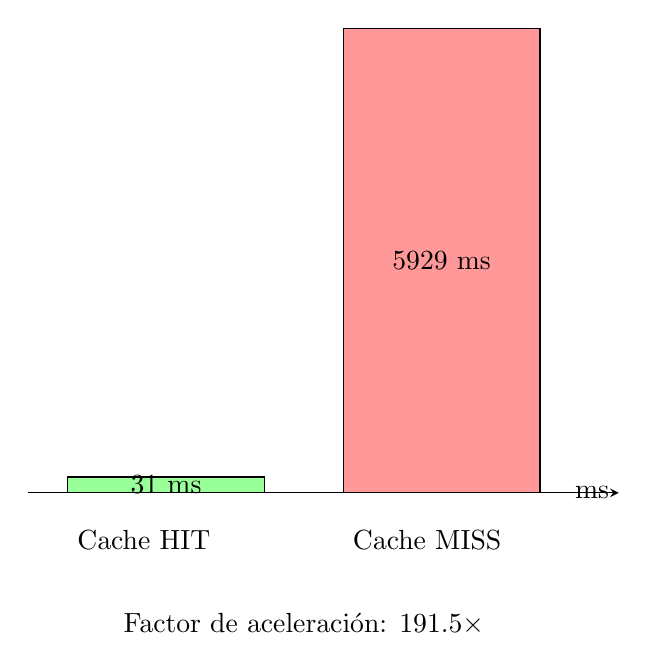
\begin{tikzpicture}
        \draw[fill=green!40]  (0,0)    rectangle (2.5,0.2)  node[midway] {31 ms};
        \draw[fill=red!40]    (3.5,0)  rectangle (6.0,5.9)  node[midway] {5929 ms};
        \node[anchor=west] at (0,-0.6)   {Cache HIT};
        \node[anchor=west] at (3.5,-0.6) {Cache MISS};
        \node[anchor=north] at (3,-1.4)  {Factor de aceleraci\'on: $191.5\times$};
        \draw[-stealth] (-0.5,0) -- (7,0);
        \node[anchor=north east] at (7,0.2) {ms};
    \end{tikzpicture}
    \caption{Latencia media de las peticiones con acierto de cach\'e (31~ms) frente a las que requieren inferencia completa (5929~ms).}
    \label{fig:latencia}
\end{figure}

\begin{figure}[H]
    \centering
    \shorthandoff{>}\shorthandoff{<}
    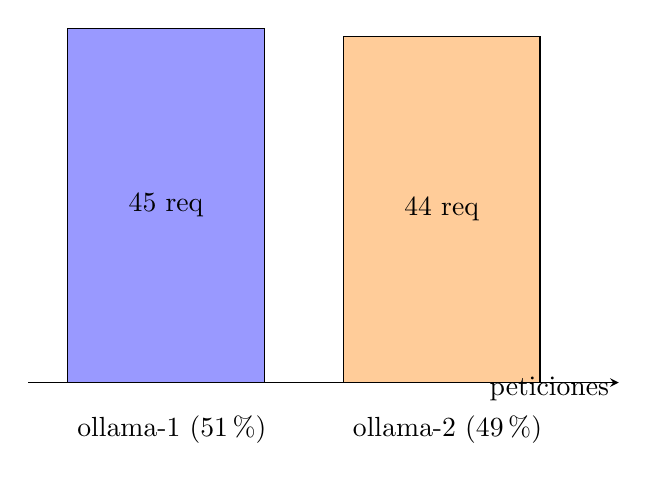
\begin{tikzpicture}
        \draw[fill=blue!40]   (0,0)   rectangle (2.5,4.5) node[midway] {45 req};
        \draw[fill=orange!40] (3.5,0) rectangle (6.0,4.4) node[midway] {44 req};
        \node[anchor=west] at (0,-0.6)   {ollama-1 (51\,\%)};
        \node[anchor=west] at (3.5,-0.6) {ollama-2 (49\,\%)};
        \draw[-stealth] (-0.5,0) -- (7,0);
        \node[anchor=north east] at (7,0.2) {peticiones};
    \end{tikzpicture}
    \caption{Distribuci\'on de 89 peticiones entre las dos instancias de inferencia.}
    \label{fig:balanceo}
\end{figure}

\subsection{Análisis de los resultados}

\textbf{Caché exacto (100\,\% de acierto).} Las 10 preguntas repetidas de forma idéntica en el grupo de duplicados exactos obtuvieron HIT en su segunda aparición sin excepción. Esto confirma que el flujo básico de almacenamiento y recuperación del caché funciona correctamente.

\textbf{Caché semántico sobre paráfrasis.} El rendimiento varía según el dominio. En Geografía, las 10 paráfrasis esperadas se detectaron correctamente (100\,\%). En Historia y Arte, 7 de 10 (70\,\%); adicionalmente se produjo un falso positivo en la primera pregunta de la Gran Muralla China (\textit{``What is the Great Wall of China?''}), que acertó en caché sin haber sido formulada antes. En Ciencia solo se detectaron 4 de 10 (40\,\%). Los falsos negativos se concentran en preguntas como las relativas a la fotosíntesis (\textit{``How does photosynthesis work?''} vs.~\textit{``Explain the process of photosynthesis''}) o la gravedad (\textit{``What is gravity?''} vs.~\textit{``How does gravity work?''}), donde el modelo de embeddings no asigna suficiente similitud coseno a pesar de la equivalencia semántica. Esto sugiere que el umbral 0.85 puede ser demasiado restrictivo para ciertos dominios.

\textbf{Falsos positivos.} Se detectó un único falso positivo en el grupo de no relacionados: la pregunta \textit{``What is the boiling point of ethanol?''} obtuvo HIT, probablemente por similitud con la pregunta \textit{``What is the boiling point of water?''} del grupo de duplicados exactos. Este caso ilustra el compromiso inherente al caché semántico: umbrales más bajos mejoran la tasa de acierto en paráfrasis a costa de aumentar los falsos positivos.

\textbf{Latencia.} La diferencia es drástica: las peticiones resueltas desde caché promedian 31~ms, frente a los 5929~ms que requiere la inferencia completa en CPU con el modelo \texttt{qwen3.5:0.8b}. El factor de aceleración es de \textbf{191.5$\times$} (mediana de 31~ms frente a 5925~ms). La latencia de caché está dominada por la generación del embedding de la pregunta entrante y la consulta al índice vectorial de Redis; la latencia de inferencia refleja el coste computacional de generar la respuesta token a token en CPU.

\textbf{Balanceo de carga.} La estrategia \texttt{simple-shuffle} produjo una distribución prácticamente equitativa: 45 peticiones a ollama-1 (51\,\%) y 44 a ollama-2 (49\,\%). La pequeña asimetría es esperable en un reparto aleatorio con un número finito de muestras.

\section{Conclusiones}

\subsection{Cumplimiento de objetivos}

Se ha construido y evaluado una granja de modelos de IA completamente funcional que integra balanceo de carga y caché semántico. El sistema se despliega de forma reproducible con un único comando (\texttt{docker compose up -d}) y expone una API compatible con OpenAI a través de un proxy Nginx.

Los resultados experimentales demuestran que:

\begin{itemize}
    \item El caché semántico proporciona una aceleración de \textbf{191.5$\times$} en latencia para preguntas repetidas o parafraseadas (31~ms frente a 5929~ms), eliminando la necesidad de ejecutar inferencia redundante.
    
    \item La detección de paráfrasis funciona correctamente en dominios con vocabulario bien diferenciado (Geografía, 100\,\%; Historia, 70\,\%), aunque presenta limitaciones en dominios técnicos como Ciencias (40\,\%).
    
    \item El balanceo de carga mediante \texttt{simple-shuffle} distribuye las peticiones de forma equitativa (51\,\%/49\,\%) sin necesidad de lógica compleja.
    
    \item La arquitectura basada en Docker Compose permite escalar horizontalmente añadiendo más instancias de Ollama, modificar el umbral de similitud o cambiar el modelo sin alterar el resto del sistema.
\end{itemize}

\subsection{Limitaciones}

El sistema presenta varias limitaciones que conviene señalar:

\begin{itemize}
    \item El umbral de similitud 0.85 es un valor fijo que no se adapta al dominio. Un umbral más bajo (0.80) habría capturado las paráfrasis de ciencia, pero podría haber generado más falsos positivos en otros grupos.
    
    \item La latencia base de inferencia (\textasciitilde6~s) está limitada por la ejecución en CPU. El uso de GPU aceleraría significativamente tanto la inferencia como la generación de embeddings.
    
    \item El sistema solo cuenta con dos réplicas de inferencia. Si ambas estuvieran saturadas, las peticiones se encolarían sin más recursos disponibles.
    
    \item El caché semántico introduce una latencia adicional en las peticiones MISS, ya que debe generar el embedding y consultar Redis antes de enviar la pregunta al modelo.
\end{itemize}

\subsection{Trabajo futuro}

A partir de los resultados obtenidos, se identifican las siguientes líneas de mejora:

\begin{enumerate}
    \item \textbf{Umbral de similitud adaptativo}: ajustar dinámicamente el umbral en función del dominio detectado en la pregunta o de la densidad de entradas en el caché, minimizando tanto falsos positivos como falsos negativos.
    
    \item \textbf{Caché multinivel}: combinar caché exacto (primer nivel, latencia $<1$~ms) con caché semántico (segundo nivel, latencia \textasciitilde31~ms), derivando al modelo solo cuando ambos fallan.
    
    \item \textbf{Más réplicas de inferencia}: añadir instancias adicionales de Ollama e implementar escalado dinámico basado en la carga observada.
    
    \item \textbf{Aceleración por hardware}: evaluar el rendimiento con GPU para inferencia y generación de embeddings, reduciendo la latencia base de \textasciitilde6~s a potencialmente cientos de milisegundos.
    
    \item \textbf{Monitorización}: integrar Prometheus y Grafana para visualizar en tiempo real la tasa de acierto de caché, latencia por percentil y distribución de carga.
    
    \item \textbf{Caché distribuido}: en un despliegue con múltiples nodos, utilizar Redis Cluster para que el caché semántico sea compartido entre todas las instancias del \textit{gateway}.
\end{enumerate}
